\documentclass[aspectratio=169,t,xcolor={dvipsnames}]{beamer}
\usepackage[english]{babel}
\usepackage[utf8]{inputenc}
\usepackage[T1]{fontenc}
\usepackage{graphicx}
\usepackage{subcaption}
\captionsetup[figure]{font=footnotesize}
\captionsetup[subfigure]{font=scriptsize}
\usepackage{hyperref}
\usepackage{booktabs}
\usepackage{amssymb}
\usepackage[binary-units]{siunitx}
\sisetup{per-mode=symbol}
\DeclareSIUnit{\frm}{frames}
\usepackage{minted}
\usepackage{tikz}
\usetikzlibrary{external,calc,positioning,fit,arrows.meta,backgrounds}

\useinnertheme[shadow=true]{rounded}
\usetheme{tud}

\institut{Institute of Computer Engineering}
\professur{Chair of Processor Design}
\title{Masterproject}
\subtitle{Partial Reconfiguration of FPGA Image Processing Pipelines with PYNQ}
\author{Tim Häring}


\begin{document}
\setbeamertemplate{caption}{\raggedright\insertcaption\par}

\maketitle

\begin{frame}{Overview}
    \begin{columns}[T]
        \begin{column}{.33\textwidth}
            \begin{block}{PYNQ}
                \begin{itemize}
                    \item High abstraction layer
                    \item Familiar to software developers
                    \item Fast development cycles
                    \item Modular design
                \end{itemize}
            \end{block}
        \end{column}
        \begin{column}{.33\textwidth}
            \begin{block}{Partial Reconfiguration}
                \begin{itemize}
                    \item Less resource utilization
                    \item Flexible and dynamically adaptive
                    \item Resilient
                \end{itemize}
            \end{block}
\begin{figure}[h]
    \centering
    \scalebox{0.37}{%
    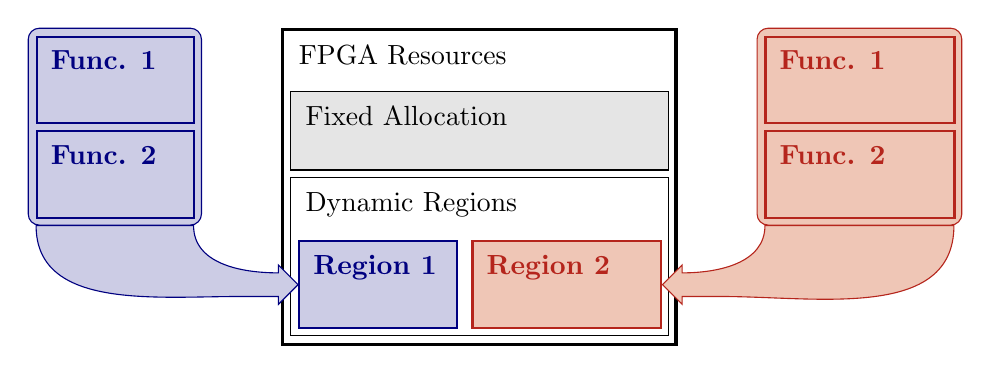
\begin{tikzpicture}
        \tikzset{dfx2/.style={minimum width=2.4cm,minimum
            height=1.1cm,fill=BrickRed!20,draw=BrickRed,thick}}
        \tikzset{dfx1/.style={minimum width=2.0cm,minimum
            height=1.1cm,fill=NavyBlue!20,draw=NavyBlue,thick}}
        \node (res) at (0,0) [draw,very thick,minimum width=5cm,minimum
            height=4cm] {};
        \node (resl) [below right=0.15cm of res.north west] {FPGA Resources};
        \node (fix) [draw,below right=0.8cm and 0.12cm of res.north west,minimum
            width=4.8cm,minimum height=1cm,fill=Gray!20] {};
        \node (fixl) [below right=0.1cm of fix.north west] {Fixed Allocation};
        \node (dyn) [draw,below right=1.9cm and 0.12cm of res.north west,minimum
            width=4.8cm,minimum height=2cm] {};
        \node (dynl) [below right=0.1cm of dyn.north west] {Dynamic Regions};
        \node (r1) [below right=0.8cm and 0.1cm of dyn.north west,dfx1] {};
        \node (r1l) [below right=0.1cm of r1.north west,color=NavyBlue]
            {\textbf{Region 1}};
        \node (r2) [below right=0.8cm and 2.3cm of dyn.north west,dfx2] {};
        \node (r2l) [below right=0.1cm of r2.north west,color=BrickRed]
            {\textbf{Region 2}};

        \node (pr1) [below left=0cm and 1cm of res.north west,minimum
            width=2.2cm,minimum
            height=2.5cm,fill=NavyBlue!20,draw=NavyBlue,rounded corners] {};
        \node (pr1f1) [below right=0.1cm and 0.1cm of pr1.north west,dfx1] {};
        \node (pr1f1l) [below right=0.1cm of pr1f1.north west,color=NavyBlue]
            {\textbf{Func. 1}};
        \node (pr1f2) [below right=1.3cm and 0.1cm of pr1.north west,dfx1] {};
        \node (pr1f2l) [below right=0.1cm of pr1f2.north west,color=NavyBlue]
            {\textbf{Func. 2}};

        \node (pr2) [below right=0cm and 1cm of res.north east,minimum
            width=2.6cm,minimum
            height=2.5cm,fill=BrickRed!20,draw=BrickRed,rounded corners] {};
        \node (pr2f1) [below right=0.1cm and 0.1cm of pr2.north west,dfx2] {};
        \node (pr2f1l) [below right=0.1cm of pr2f1.north west,color=BrickRed]
            {\textbf{Func. 1}};
        \node (pr2f2) [below right=1.3cm and 0.1cm of pr2.north west,dfx2] {};
        \node (pr2f2l) [below right=0.1cm of pr2f2.north west,color=BrickRed]
            {\textbf{Func. 2}};

        \filldraw [fill=NavyBlue!20,draw=NavyBlue] let \p1 = (pr1.south), \p2 =
            (r1.west) in (\x2,\y2) -- ++(-0.25,-0.25) -- ++(0,0.1) -- ++(-0.5,0)
            to [out=180,in=270] (\x1 - 1cm,\y1) -- (\x1 + 1cm,\y1) to
            [out=270,in=180] (\x2 - 0.25cm, \y2 + 0.15cm) -- ++(0,0.1) -- cycle;

        \filldraw [fill=BrickRed!20,draw=BrickRed] let \p1 = (pr2.south), \p2 =
            (r2.east) in (\x2,\y2) -- ++(0.25,-0.25) -- ++(0,0.1) -- ++(0.5,0)
            to [out=0,in=270] (\x1 + 1.2cm,\y1) -- (\x1 - 1.2cm,\y1) to
            [out=270,in=0] (\x2 + 0.25cm, \y2 + 0.15cm) -- ++(0,0.1) -- cycle;
    \end{tikzpicture}
}
    \caption{DPR resource usage.}%
    \label{fig:reconf}%
\end{figure}
        \end{column}
        \begin{column}{.33\textwidth}
            \begin{block}{Image Processing}
                \begin{itemize}
                    \item Widely used
                    \item Algorithms with similar structure
                    \item \texttt{xfOpenCV} library for HLS synthesis
                \end{itemize}
            \end{block}
        \end{column}
    \end{columns}
\end{frame}


\begin{frame}{Framework}
    \begin{columns}[T]
        \begin{column}{.45\textwidth}
\begin{figure}[h]
    \centering
    \scalebox{0.5}{%
    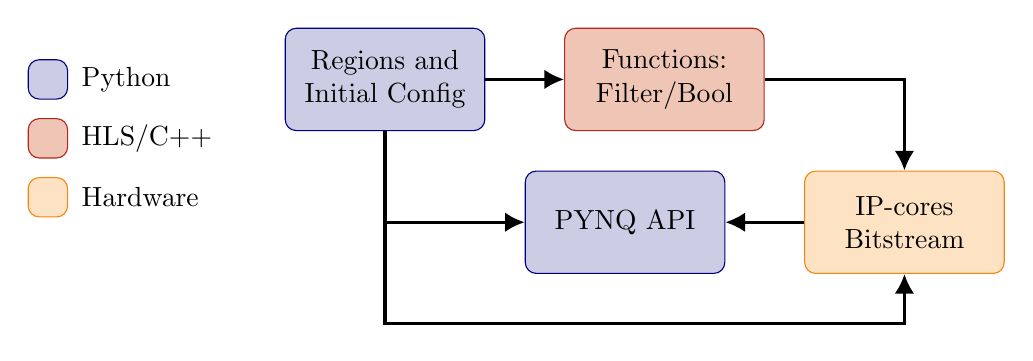
\begin{tikzpicture}
        \tikzset{node/.style={rounded corners,minimum
            height=1.3cm,align=center,text width=2.3cm}}
        \tikzset{leg/.style={rounded corners,minimum
            height=0.5cm,minimum width=0.5cm}}
        \tikzset{python/.style={fill=NavyBlue!20,draw=NavyBlue,node}}
        \tikzset{hls/.style={fill=BrickRed!20,draw=BrickRed,node}}
        \tikzset{ip/.style={fill=BurntOrange!20,draw=BurntOrange,node}}
        \tikzset{pythonl/.style={fill=NavyBlue!20,draw=NavyBlue,leg}}
        \tikzset{hlsl/.style={fill=BrickRed!20,draw=BrickRed,leg}}
        \tikzset{ipl/.style={fill=BurntOrange!20,draw=BurntOrange,leg}}
        \tikzset{arr/.style={-{Latex[length=0.25cm,width=0.25cm]},line
            width=.04cm}}

        \node (p) at (0,0) [python] {Regions and\\Initial Config};
        \node (h) [right=of p,hls] {Functions:\\Filter/Bool};
        \node (i) [below right=0.5cm and 0.5cm of h,ip]
            {IP-cores\\Bitstream};
        \node (pynq) [below right=0.5cm and 0.5cm of p,python] {PYNQ API};
        \node (help) [below=0.5cm of i] {};

        \node (legp) at (-4,0) {};
        \node [left=-0.1cm of legp,pythonl] {};
        \node [right=-0.1cm of legp] {Python};
        \node (legh) [below=0.5cm of legp] {};
        \node [left=-0.1cm of legh,hlsl] {};
        \node [right=-0.1cm of legh] {HLS/C++};
        \node (legi) [below=0.5cm of legh] {};
        \node [left=-0.1cm of legi,ipl] {};
        \node [right=-0.1cm of legi] {Hardware};

        \draw [arr] (p.south) |- (pynq.west);
        \draw [arr] (p.east) -- (h.west);
        \draw [arr] (h.east) -| (i.north);
        \draw [arr] (i.west) -- (pynq.east);
        \draw [arr] let \p1 = (p.south), \p2 = (help), \p3 = (i.south) in
            (\x1,\y1) -- (\x1,\y2) -- (\x2,\y2) -- (\x3,\y3);
    \end{tikzpicture}
}
    \caption{Framework components overview.}%
    \label{fig:approach}%
\end{figure}
        \end{column}
        \begin{column}{.5\textwidth}
            \begin{block}{Implemented Components}
                \begin{itemize}
                    \item Python and \texttt{.tcl} scripts
                    \item C++ filter implementations for HLS
                    \item Automatic generation of hardware
                    \item No PYNQ bindings, use \texttt{allocate}
                    \item Fixed HW communication paths
                \end{itemize}
            \end{block}
        \end{column}
    \end{columns}
\end{frame}


\begin{frame}{Algorithm}
    \begin{columns}[T]
        \begin{column}{.45\textwidth}
\begin{figure}[h]
    \centering
    \scalebox{0.42}{%
    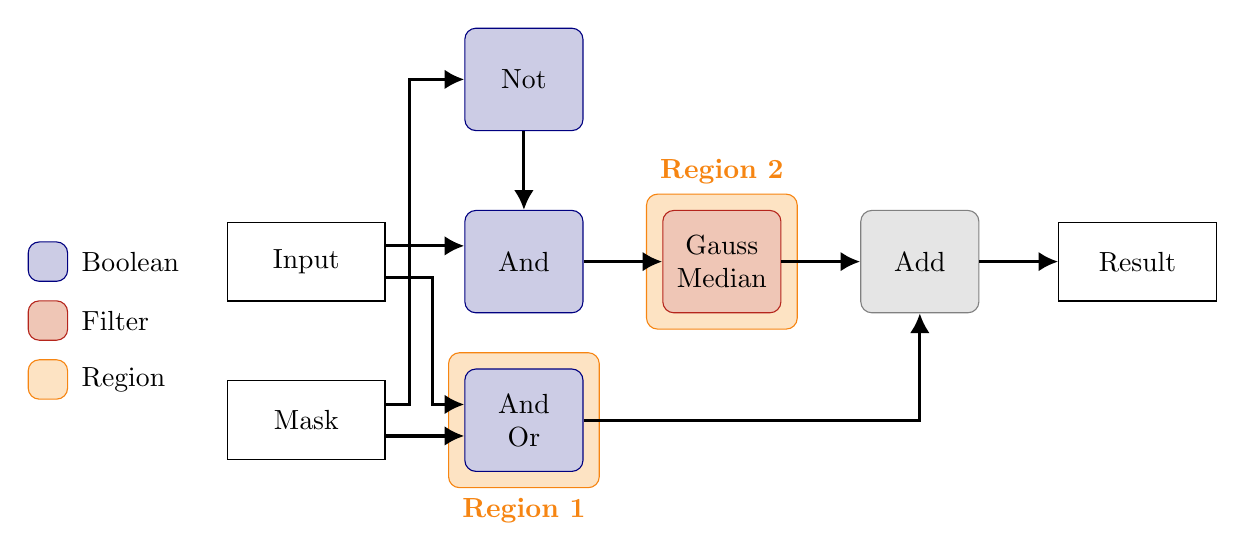
\begin{tikzpicture}
        \tikzset{img/.style={draw,minimum width=2.0cm,minimum height=1.0cm}}
        \tikzset{node/.style={rounded corners,minimum width=1.5cm,minimum
            height=1.3cm,align=center}}
        \tikzset{reg/.style={rounded corners,inner sep=0.2cm}}
        \tikzset{leg/.style={rounded corners,minimum width=0.5cm,minimum
            height=0.5cm}}
        \tikzset{bool/.style={fill=NavyBlue!20,draw=NavyBlue,node}}
        \tikzset{addn/.style={fill=Gray!20,draw=Gray,node}}
        \tikzset{filter/.style={fill=BrickRed!20,draw=BrickRed,node}}
        \tikzset{region/.style={fill=BurntOrange!20,draw=BurntOrange,reg}}
        \tikzset{booll/.style={fill=NavyBlue!20,draw=NavyBlue,leg}}
        \tikzset{filterl/.style={fill=BrickRed!20,draw=BrickRed,leg}}
        \tikzset{regionl/.style={fill=BurntOrange!20,draw=BurntOrange,leg}}
        \tikzset{arr/.style={-{Latex[length=0.25cm,width=0.25cm]},line
            width=.04cm}}

        \node (input) at (0,0) [img] {Input};
        \node (mask) [below=of input,img] {Mask};
        \node (bool1) [right=of mask,bool] {And\\Or};
        \node (bool2) [right=of input,bool] {And};
        \node (not) [above=of bool2,bool] {Not};
        \node (filter) [right=of bool2,filter] {Gauss\\Median};
        \node (add) [right=of filter,draw,addn] {Add};
        \node (res) [right=of add,img] {Result};

        \node (legb) at (-3,0) {};
        \node [left=-0.1cm of legb,booll] {};
        \node [right=-0.1cm of legb] {Boolean};
        \node (legf) [below=0.5cm of legb] {};
        \node [left=-0.1cm of legf,filterl] {};
        \node [right=-0.1cm of legf] {Filter};
        \node (legr) [below=0.5cm of legf] {};
        \node [left=-0.1cm of legr,regionl] {};
        \node [right=-0.1cm of legr] {Region};

        \begin{scope}[on background layer]
            \node (r1) [region,fit=(bool1)] {};
            \node [below=0cm of r1,color=BurntOrange] {\textbf{Region 1}};
            \node (r2) [region,fit=(filter)] {};
            \node [above=0cm of r2,color=BurntOrange] {\textbf{Region 2}};
        \end{scope}

        \draw [arr] let \p1 = (input.east), \p2 = (bool1.west) in
            (\x1,\y1-0.2cm) -- ++(0.6cm,0) |- (\x2,\y2+0.2cm);
        \draw [arr] let \p1 = (mask.east), \p2 = (bool1.west) in (\x1,\y1-0.2cm)
            -- (\x2,\y2-0.2cm);
        \draw [arr] let \p1 = (mask.east), \p2 = (not.west) in (\x1,\y1+0.2cm)
            -- ++(0.3cm,0) |- (\x2,\y2);
        \draw [arr] (not.south) -- (bool2.north);
        \draw [arr] let \p1 = (input.east), \p2 = (bool2.west) in
            (\x1,\y1+0.2cm) -- (\x2,\y2+0.2cm);
        \draw [arr] (bool2.east) -- (filter.west);
        \draw [arr] (filter.east) -- (add.west);
        \draw [arr] (bool1.east) -| (add.south);
        \draw [arr] (add.east) -- (res.west);
    \end{tikzpicture}
}
    \caption{Implemented processing pipeline.}%
    \label{fig:func}%
\end{figure}
        \end{column}
        \begin{column}{.5\textwidth}
            \begin{block}{Overlays}
                \begin{itemize}
                    \item Base: And/Median \& Or/Gauss
                    \item Streaming: no DMA
                    \item Partial: reconfiguration regions
                    \item Software: Cortex-A9@\SI{650}{\mega\hertz}
                \end{itemize}
            \end{block}
            \begin{block}{Benchmarking Parameters}
                \begin{itemize}
                    \item \SI{100}{\mega\hertz} hardware clock
                    \item Full HD images ($\approx\SI{2}{\mega\byte}$)
                \end{itemize}
            \end{block}
        \end{column}
    \end{columns}
\end{frame}


\begin{frame}{Results}
\begin{figure}[h]
    \centering
    \begin{subfigure}{.3\textwidth}
        \centering
        \includegraphics[width=0.9\linewidth]{../../python/person}
        \subcaption{Input Image}%
        \label{subfig:input}
    \end{subfigure}\hfill
    \begin{subfigure}{.3\textwidth}
        \centering
        \includegraphics[width=0.9\linewidth]{../../python/and_gauss_81}
        \subcaption{And/Gauss}%
        \label{subfig:input}
    \end{subfigure}\hfill
    \begin{subfigure}{.3\textwidth}
        \centering
        \includegraphics[width=0.9\linewidth]{../../python/and_median_81}
        \subcaption{And/Median}%
        \label{subfig:input}
    \end{subfigure}\hfill
    \medskip
    \begin{subfigure}{.3\textwidth}
        \centering
        \includegraphics[width=0.9\linewidth]{../../python/mask_big}
        \subcaption{Mask}%
        \label{subfig:input}
    \end{subfigure}\hfill
    \begin{subfigure}{.3\textwidth}
        \centering
        \includegraphics[width=0.9\linewidth]{../../python/or_gauss_81}
        \subcaption{Or/Gauss}%
        \label{subfig:input}
    \end{subfigure}\hfill
    \begin{subfigure}{.3\textwidth}
        \centering
        \includegraphics[width=0.9\linewidth]{../../python/or_median_81}
        \subcaption{Or/Median}%
        \label{subfig:input}
    \end{subfigure}\hfill
    \caption{Inputs and results of the processing pipeline.}%
    \label{fig:images}%
\end{figure}
\end{frame}


\begin{frame}{Results --- Resource Utilization}
    \begin{columns}[T]
        \begin{column}{.5\textwidth}
\begin{table}[h]
    \centering
    \begin{tabular}{l S S S}
        \toprule
         & {Slice LUT} & {BRAM} & {DSP} \\
        {Overlay} & [\si{\percent}] & [\si{\percent}] & [\si{\percent}] \\
        \midrule
        Base        & 54.52 &  9.29 & 35.45 \\
        Streaming   & 62.43 & 16.43 & 12.18 \\
        Partial     & 31.78 &  5.36 & 10.91 \\
        \bottomrule
    \end{tabular}
    \caption{Resource utilization percentage of the implemented overlays.}%
    \label{tab:res}%
\end{table}
        \end{column}
        \begin{column}{.45\textwidth}
            \begin{block}{Overlay Results}
                \begin{itemize}
                    \item Base: two pipelines in parallel
                    \item Streaming: additional HDMI processing overhead
                    \item Partial: shows advantages of partial reconfiguration
                \end{itemize}
            \end{block}
        \end{column}
    \end{columns}
\end{frame}


\begin{frame}{Results --- Performance}
    \begin{columns}[T]
        \begin{column}{.5\textwidth}
\begin{table}[h]
    \centering
    \begin{tabular}{l S S}
        \toprule
        & {Latency} & {Performance} \\
        Overlay & [\si{\milli\second}] & [\si{\frm\per\second}] \\
        \midrule
        Base        &  22.73 & 43.98 \\
        Streaming   &  20.83 & 48.00 \\
        Partial     &  23.35 & 42.82 \\
        \midrule
        Software    & 365.03 &  2.73 \\
        \bottomrule
    \end{tabular}
    \caption{Performance results of different implementations.}%
    \label{tab:perf}%
\end{table}
        \end{column}
        \begin{column}{.45\textwidth}
            \begin{block}{Implementation Results}
                \begin{itemize}
                    \item Base: two pipelines in parallel
                    \item Streaming: no DMA access
                    \item Partial: reconfiguration takes $\approx
                        \SI{200}{\milli\second} \Rightarrow \SI{10}{\frm}$
                    \item Software: little processing power $\Rightarrow$
                        HW acceleration
                \end{itemize}
            \end{block}
        \end{column}
    \end{columns}
\end{frame}


\begin{frame}{Conclusion}
    \begin{columns}[T]
        \begin{column}{.45\textwidth}
            \begin{block}{Achieved}
                \begin{itemize}
                    \item Simple hardware acceleration framework ($\times 15$)
                    \item Easily usable by software developers through PYNQ
                    \item Extension/HW modification requires HW knowledge
                    \item Fixed communication paths
                \end{itemize}
            \end{block}
        \end{column}
        \begin{column}{.45\textwidth}
            \begin{block}{Outlook}
                \begin{itemize}
                    \item Integrate DPR into streaming overlay (no DMA required)
                    \item Extend with NOC
                \end{itemize}
            \end{block}
        \end{column}
    \end{columns}
\end{frame}


\begin{frame}{Questions?}
\end{frame}
\end{document}

%%% Local Variables:
%%% mode: latex
%%% TeX-command-extra-options: "-shell-escape"
%%% End:
